

\chapter{Introduction}
\label{chap:intro_vhdl}

\section{Why HDL}
\label{sec:why_hdl}


Before starting learning \verb|VHDL|, let's see the idea behind \verb|HDL| in general. Consider a mux circuit shown in \autoref{fig:intro_hdl:mux_circuit}.


\begin{figure}[h]
\centering
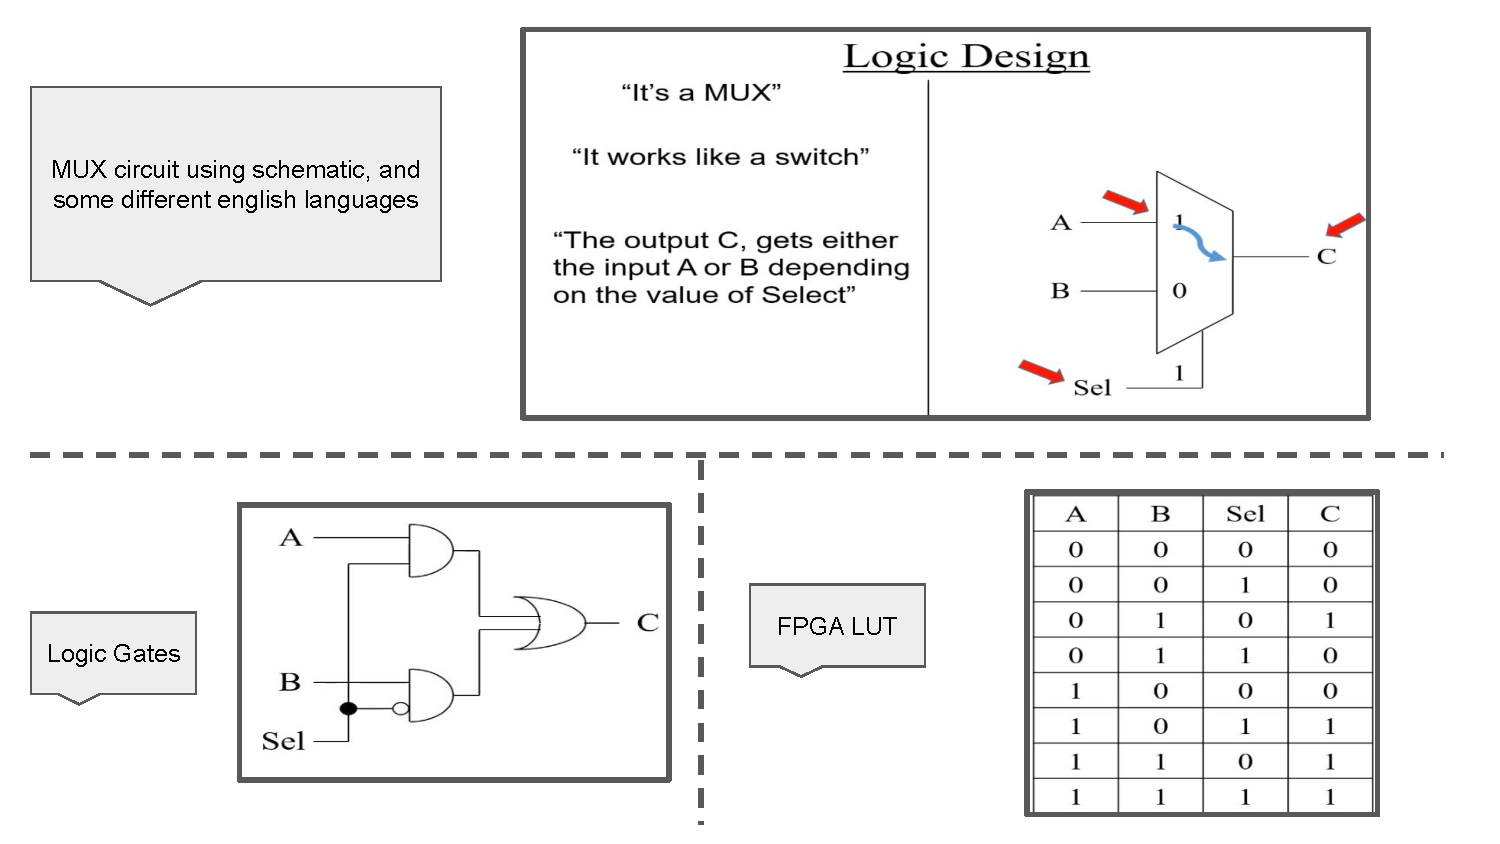
\includegraphics[scale=0.6,frame]{Figures/intro_hdl/mux_circuit}
\caption{Different method to describe a MUX circuit}
\label{fig:intro_hdl:mux_circuit}
\end{figure}

A MUX can be described using english languages, or the logic gates behind it, or even by LUT. But all these methods are somehow not practical when dealing with some complex design.

The other method which is better to implement our desing is to give some behaviour for the desing (function), and let the tools figure out what logic needs to be used. As long as the tools implement correctly the behaviour, we don't care about the underlying logic. This is the basic idea behind \verb|HDL| such as \verb|VHDL| and \verb|Verilog|.

\newpage
\subsection{Desing methodolgies}
\label{sub:desing_evolution}

Throughout time, desing evolves through 3 phases:

\begin{figure}[h]
\centering
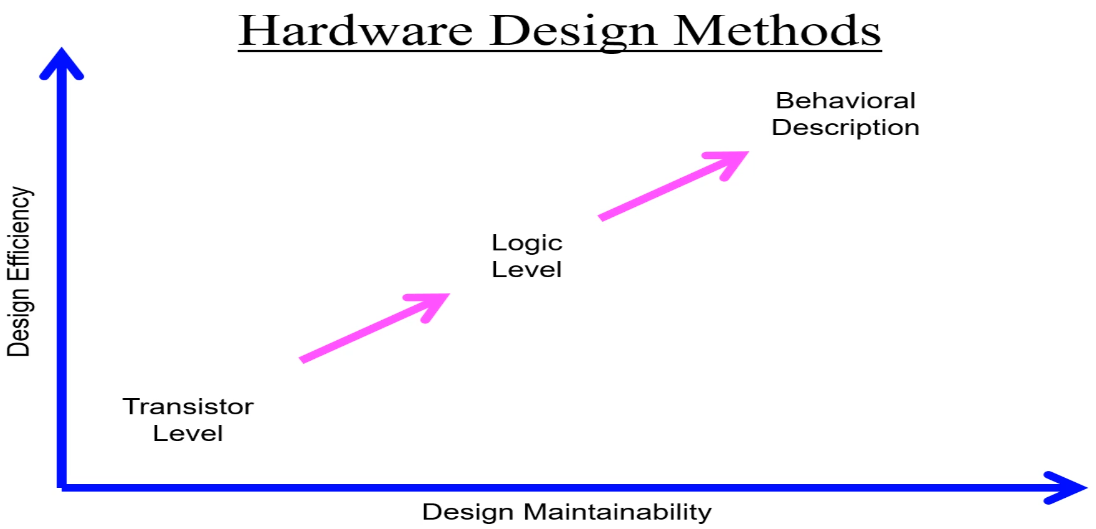
\includegraphics[scale=0.4,frame]{Figures/intro_hdl/design_evol}
\caption{Desing evolution}
\label{fig:intro_hdl:design_evol}
\end{figure}

\begin{itemize}

\item Connecting transistors manually

\item Then use symbol and schematic to simplify the manual connections

	\begin{itemize}
	\item Such in digital desing courses
	\end{itemize}

\item Then move to \verb|HDL| and let the tools figure out the gates and the schematic

\end{itemize}

\subsection{VHDL}

\verb|VHDL| was created in United states as some defense project for electronic simulation, then later used in logic modeling and simulation.


The most common standard used today is 1993, and recent standard are added after revision in 2006 and 2008.\\

\newpage
\underline{Simulation and Synthesis:}\\

\verb|VHDL| is a language used for simulation and modeling, and there is allot of features that can't be used in synthesis.

\begin{figure}[h]
\centering
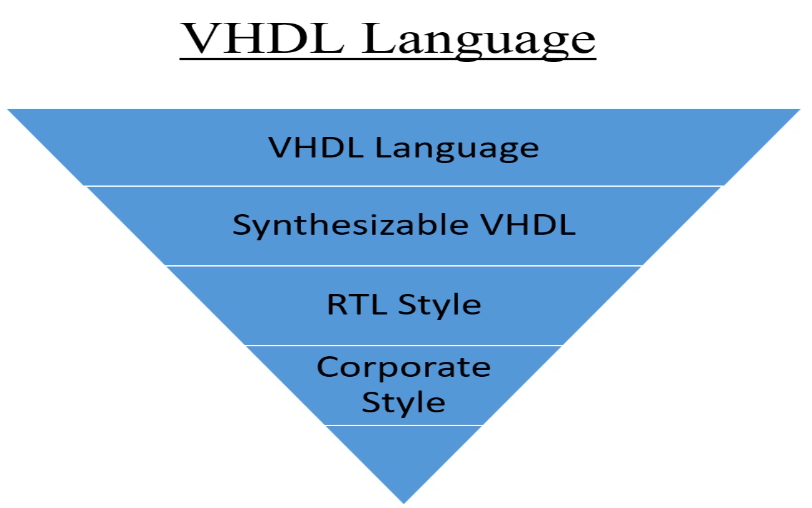
\includegraphics[scale=0.4,frame]{Figures/intro_hdl/vhdl_organisation}
\caption{VHLD different sets of the language}
\label{fig:intro_hdl:vhdl_organisation}
\end{figure}


There is a subset of the language used for synthesis, and we have a specific style used for the logic synthesis called \textit{RTL style}, which will be the focus of this course.

In companies, it is also common to have to whay is called \textit{corporate style}, that is some coding style specific to that company which uses features in certain way. In this course, we focus on Boing style.


\newpage
\subsection{FPGA}

FPGA is a device composed of many cells, where each cells contains many LUT and FF. The complexity of an FPGA resides in the millions of ways to connect LUT and FF \textit{wihting a cell} and \textit{between cells also}. We use \verb|HDL| and let the tools figures out these connections.

\begin{figure}[h]
\centering
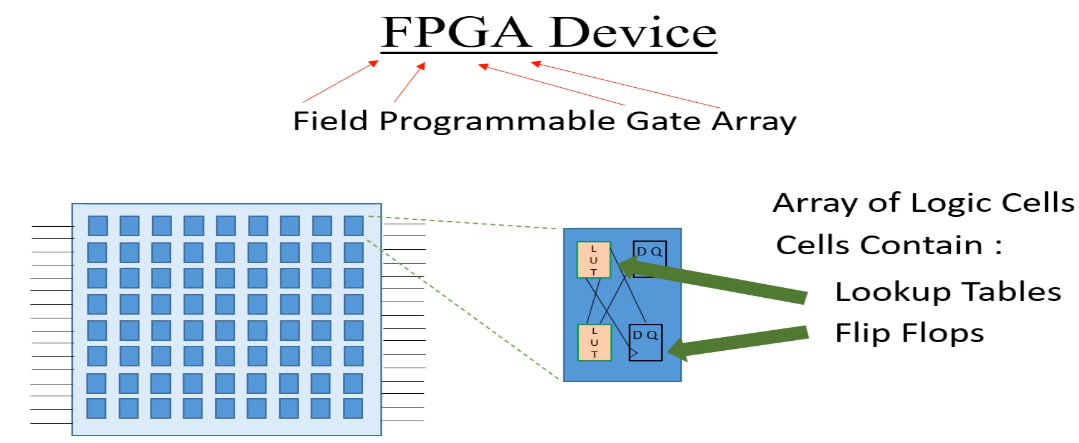
\includegraphics[scale=0.33,frame]{Figures/intro_hdl/fpga_dev}
\caption{FPGA device}
\label{fig:intro_hdl:fpga_dev}
\end{figure}


\subsection{FPGA Configuration}
\label{sub:fpga_conf}

By FPGA configuration we mean the way the interconnection is made within the logic cell it self, and from 1 cell to another. This is done by loading these information using some static RAM (or any type of memory), where the SRAM can be transfer using flash memory, or JTAG cable, or some through some processor protocol like \verb|SPI|.

Once these configuration are transfer to make the connections, the connections are made throughout some siwthch boxes, within the cell itself, and from 1 cell to another.

\begin{figure}[h]
\centering
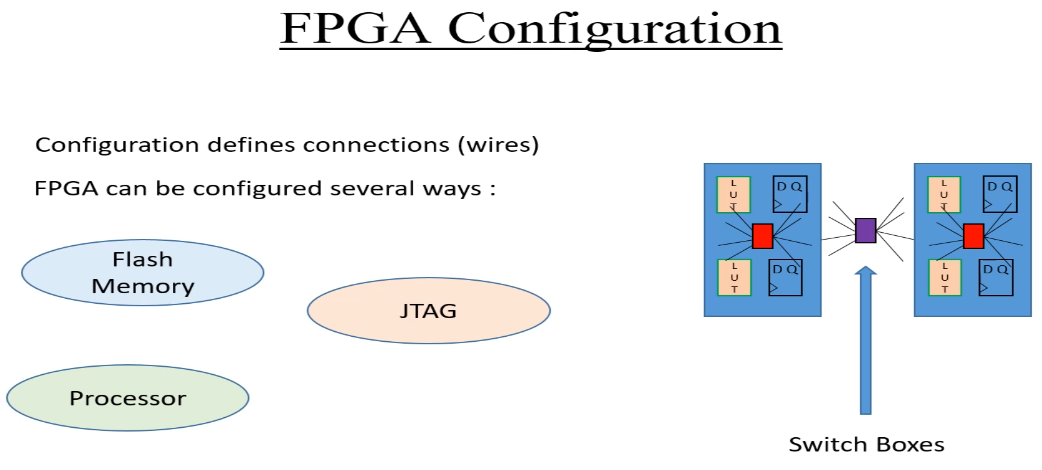
\includegraphics[scale=0.33,frame]{Figures/intro_hdl/fpga_conf}
\caption{FPGA device}
\label{fig:intro_hdl:fpga_conf}
\end{figure}

This step is defined and implemented is the $\mathrm{3}^\mathrm{rd}$ step of the FGPA desing flow (\ref{sec:desing_flow}), called \textit{place and route}.


\newpage
\section{Desing Flow}
\label{sec:desing_flow}

Now we turn to the FPGA development process. We have 3 phases, as shown in \autoref{fig:intro_hdl:fpga_development_process}.

\begin{figure}[h]
\centering
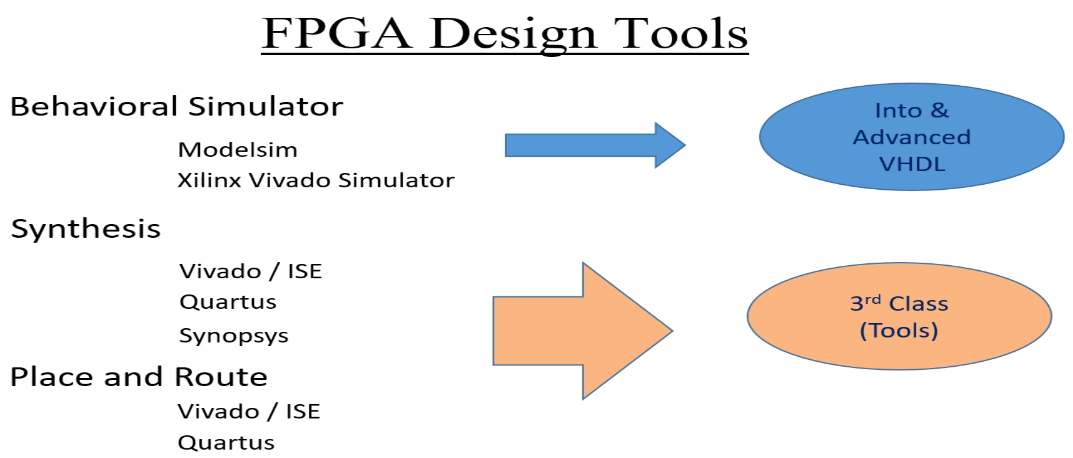
\includegraphics[scale=0.4,frame]{Figures/intro_hdl/fpga_development_process}
\caption{FPGA development process}
\label{fig:intro_hdl:fpga_development_process}
\end{figure}


\begin{itemize}

\item The $\mathrm{1}^\mathrm{st}$ step is the \textit{behavioral simulator}, that is we simulate behavioral description of our desing using tools such as \verb|Modelsim| or \verb|Vivado| from \verb|AMD|. 

\item Once we make sure that the desing simulate the behavior correctly, we translate the behavioral description into logic.

This is done using \textit{synthesis tools}, such as \verb|Vivado| also.

\item $\mathrm{3}^\mathrm{rd}$ step: place and route

\end{itemize}

\subsection{Behavioral Simulation}
\label{sub:behaviour_sim}

In the $\mathrm{1}^\mathrm{st}$ part of the course, we will focus on behaviour simulation.\\

The idea behind behavioral simulation is that we are simulating the behaviour of the \verb|VHDL| code, and not the logic synthesised yet. 

This is done using waveform visualisation, that is giving our code a set of input (stimulus), and then we hope that our code produce the correct result, and be able to visulaize this using the waveforms.


\begin{figure}[h]
\centering
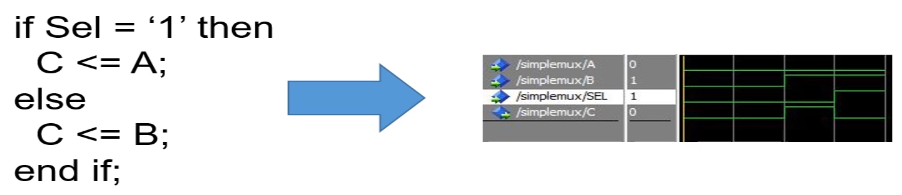
\includegraphics[scale=0.4,frame]{Figures/intro_hdl/behaviour_sim}
\caption{Behavioural simulation by using waveforms and set of stimulus}
\label{fig:intro_hdl:behaviour_sim}
\end{figure}

\newpage

\subsection{Gate Level Simulation}

This is the part we simulate tha actual logic synthesis by the tools. The goal is to hope that gate simulation mathces the behaviour simulations. It is always better to do both, and with experience we gain some confidence that our \verb|HDL| code produces the correct gate simulaitons.

\begin{figure}[h]
\centering
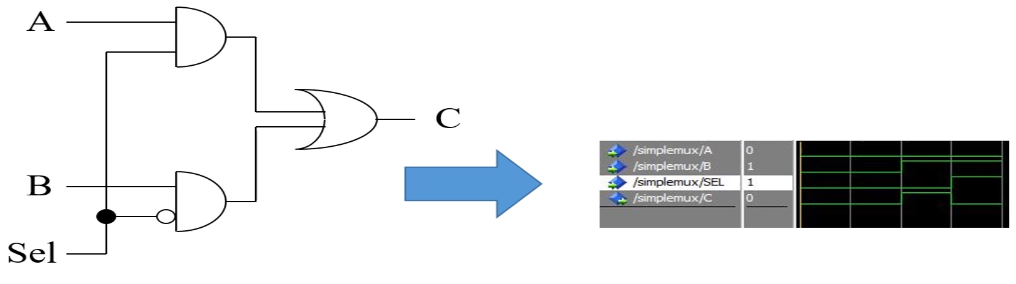
\includegraphics[scale=0.28,frame]{Figures/intro_hdl/gate_sim}
\caption{Gate level simulation: output produce by actual gates}
\label{fig:intro_hdl:gate_sim}
\end{figure}

\underline{What can go wrong?}

\begin{itemize}

\item Sometimes we describe things that can't be translated into logic

\item After synthesis, timing problems.

	\begin{itemize}
	\item We learn how to correct these issues in another part of the course 
	\end{itemize}

\end{itemize}

\subsection{Wrapping up the desing flow}

\autoref{fig:intro_hdl:desing_flow_sequence} presents another view of the development process seen in \autoref{fig:intro_hdl:fpga_development_process}.

\begin{figure}[h]
\centering
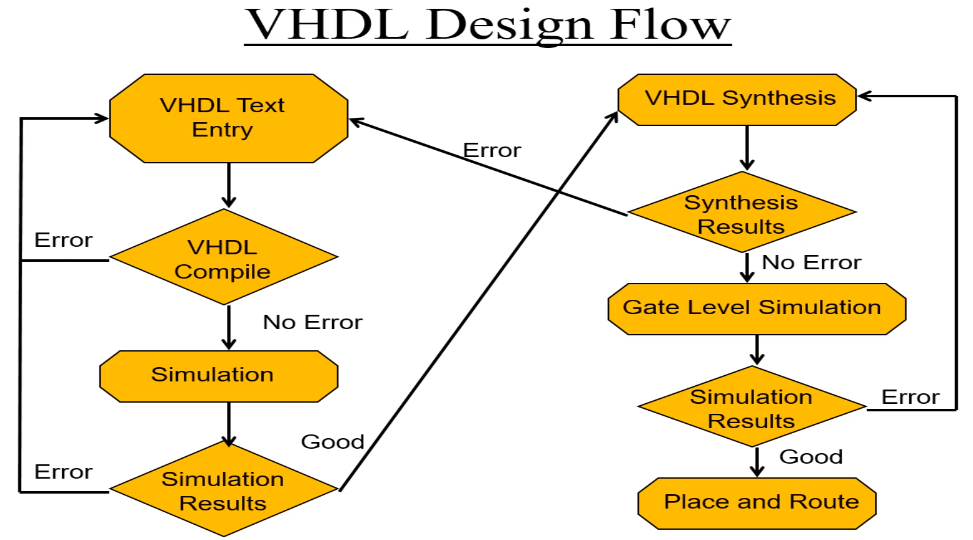
\includegraphics[scale=0.4,frame]{Figures/intro_hdl/desing_flow_sequence}
\caption{Desing flow}
\label{fig:intro_hdl:desing_flow_sequence}
\end{figure}

\begin{itemize}

\item Before the running the simulation part (behavioural simulation as see in \ref{sub:behaviour_sim}), there is the compilation step where we can check for errors like syntax errors, langauges rules,$\cdots$

\item Same concept for gate level simulation, we have to pass also the synthesis result step

\end{itemize}



\newpage
\section{VHDL is not a software}
\label{sub:vhdl_nature}

It is important to keep in mind is not a traditional programming language, that is the final output is not binary or some executable like a \verb|C| program, which runs on some machine. As a matter of fact, we need to think of \verb|VHDL| as some kind of desing tools which let us \textit{describe the behaviour of our desing}, and then using vendors tools we synthesis this behavour into actual gates and circuit.

\begin{figure}[h]
\centering
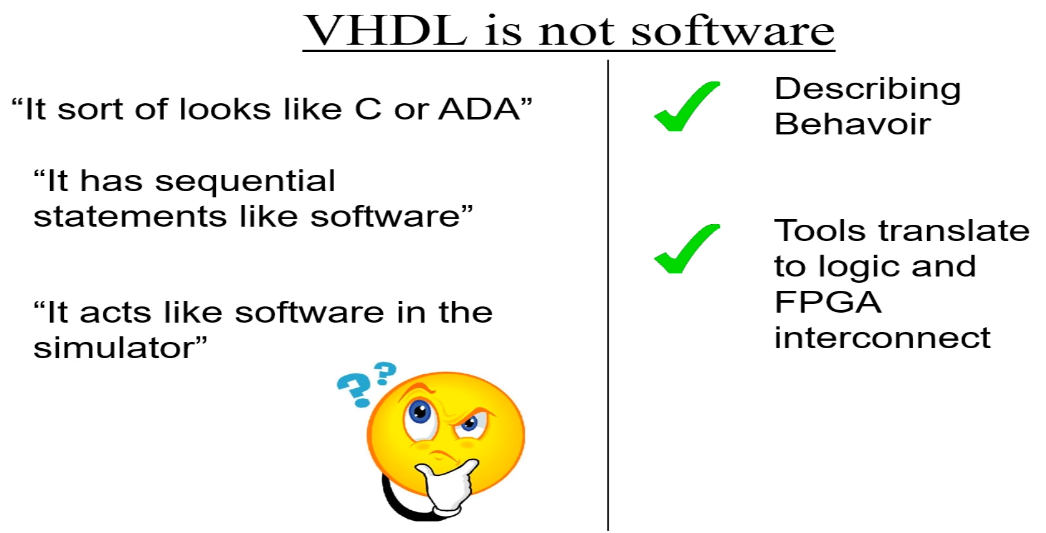
\includegraphics[scale=0.4,frame]{Figures/intro_hdl/vhdl_concept}
\caption{VHDL concept}
\label{fig:intro_hdl:vhdl_concept}
\end{figure}

So in other words, \verb|VHDL| is a tools which produces circuit, and not some binary.

After experience, we can imagine what is the circuit behind our \verb|VHDL| code lines .


\newpage
\section{VHDL Desing}
\label{sec:vhdl_desing}

Now we move more toward the desing itself and \verb|VHDL| language.\\

There are 2 blocks to have a correct \verb|VHDL| module as seen in \autoref{fig:intro_hdl:vhdl_component}:

\begin{figure}[h]
\centering
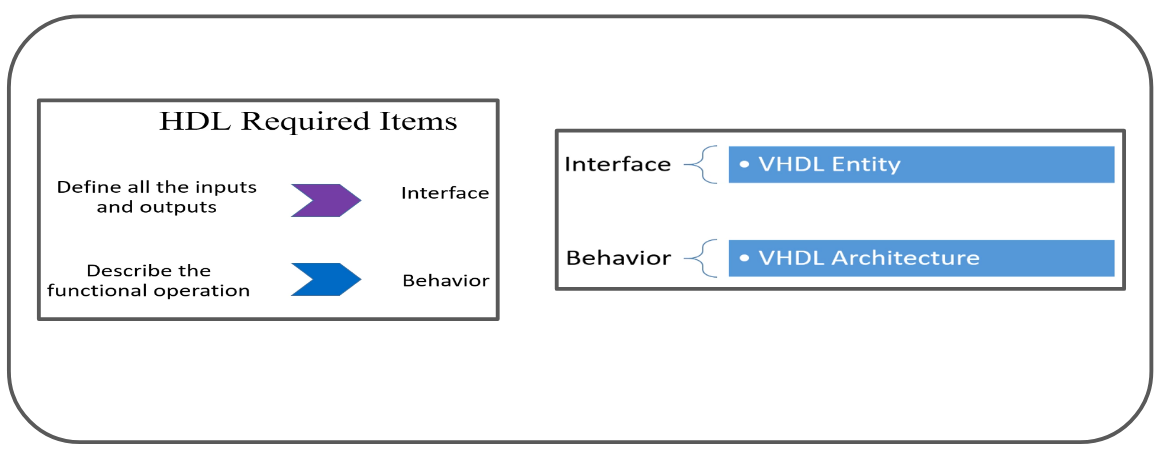
\includegraphics[scale=0.4,frame]{Figures/intro_hdl/vhdl_component}
\caption{VHDL component}
\label{fig:intro_hdl:vhdl_component}
\end{figure}

\begin{itemize}

\item The input and output part, which are structured in \textit{entity} unit

\item The behavioral part, that is the actual work of the system, and it is contained in \textit{architecture} unit

\end{itemize}

In \verb|VHDL| vocab, a complete \verb|VHDL| desing which is formed by an entity and a architecture is called \textit{component}.

\subsection{Entity}

The entity contains all input output of our desing. \autoref{fig:intro_hdl:vhdl_entity} shows the parameter and syntax of \verb|VHDL| entity


\begin{figure}[h]
\centering
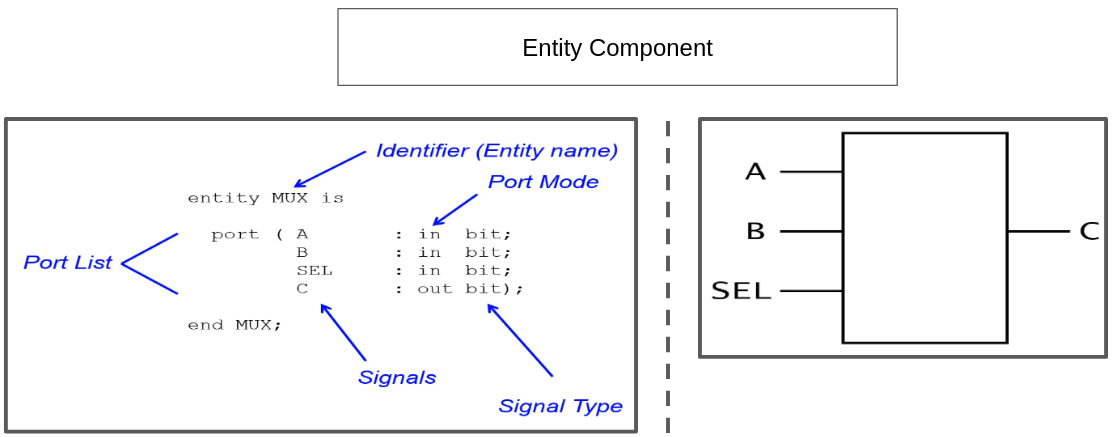
\includegraphics[scale=0.4,frame]{Figures/intro_hdl/vhdl_entity}
\caption{VHDL entity}
\label{fig:intro_hdl:vhdl_entity}
\end{figure}

\begin{itemize}

\item We begin by the keyword \verb|entity| and its name (\verb|MUX|)

\item \verb|port()| contains a list of all input and output

\item we type their name (\verb|A|) followed by \verb|:|

\item Their mode \verb|in| or \verb|out|

\item Their type \verb|bit|

\item Finally we use the \verb|end| and the name \verb|MUX|

\end{itemize}

\underline{Some notes:}

\begin{itemize}

\item In \verb|VHDL|, an entity must be associated with some architecture, where we code our behaviour.

\item From a syntax: note that in \autoref{fig:intro_hdl:vhdl_entity} that the last \verb|;| is placed after the parenthesis, and not before

\end{itemize}

\subsection{Architecture}
 
The architecture is where we define our functional desing. 
 
\begin{figure}[h]
\centering
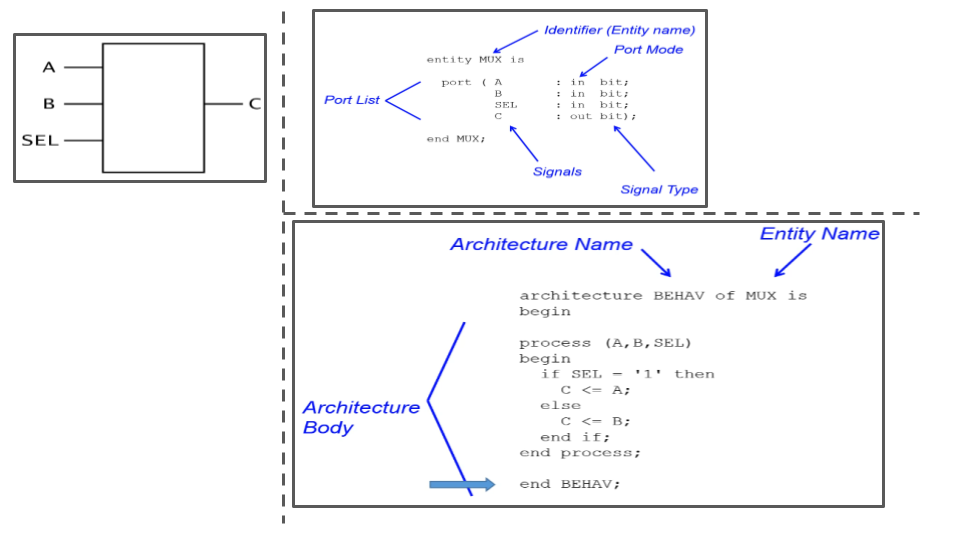
\includegraphics[scale=0.4,frame]{Figures/intro_hdl/vhdl_archi}
\caption{VHDL architecture with its corresponding entity}
\label{fig:intro_hdl:vhdl_archi}
\end{figure} 
 
\begin{itemize}

\item The $\mathrm{1}^\mathrm{st}$ line is the \textit{architecture declaration}, where we have the archi name (\verb|BEHAV|) and the associated entity (\verb|MUX|)

\item After declaration, we use the keyword \verb|begin|

	\begin{itemize}
	\item Inside this \verb|begin| block, we put our code, that is the behavioural description of our system
	\end{itemize}

\item In the case of a MUX circuit, we put our behavioral description inside \verb|process| block, where we have some sequential statemets, that is statement executed one after another

\end{itemize} 
 

\subsection{Internal Signals}
\label{sub:internal_sig}

Any signal (like a variable) wich is defined in the entity can be used inside the archtiecture. However, sometimes we can use some internal signals, that is signal which are only visibile inside the architecture unit. An example is shown in \autoref{fig:intro_hdl:int_sig_ex}.


\begin{figure}[h]
\centering
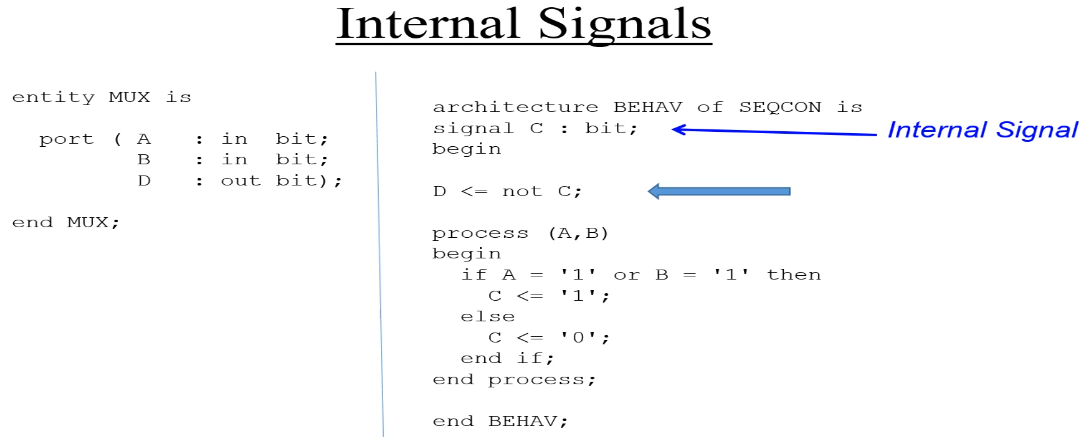
\includegraphics[scale=0.4,frame]{Figures/intro_hdl/int_sig_ex}
\caption{Internal signal example}
\label{fig:intro_hdl:int_sig_ex}
\end{figure} 

\begin{itemize}

\item signal \verb|C| is declared inside the architecture, but in the entity

\item It is assigned to \verb|D| by wiring up to a \verb|NOT| gate

\item Then it is executed both in parallel with the process

\end{itemize}

\newpage
\subsection{Concurrency}
\label{sub:concurrency}

The statement defined outside a process but inside the architecture are executed in parallel with the processes. \autoref{fig:intro_hdl:and_gate_seq_vs_conc} present an example of \verb|AND| implementation


\begin{figure}[h]
\centering
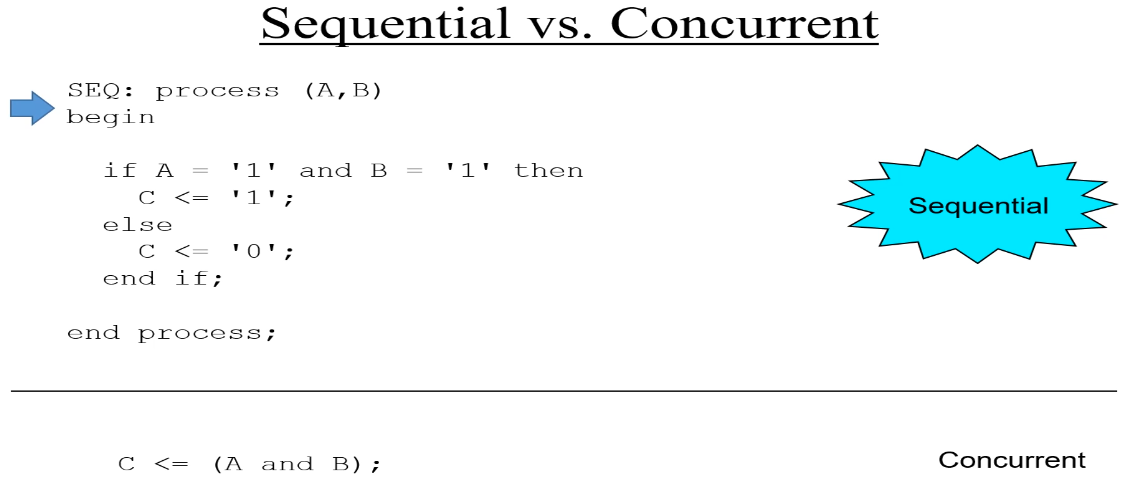
\includegraphics[scale=0.35,frame]{Figures/intro_hdl/and_gate_seq_vs_conc}
\caption{and gate implementation using sequential and concurent style}
\label{fig:intro_hdl:and_gate_seq_vs_conc}
\end{figure} 

\begin{itemize}

\item $\mathrm{1}^\mathrm{st}$ implementation sequential style using \verb|if-else|

\item $\mathrm{2}^\mathrm{nd}$ style using \verb|and| keyword statement , which is concurrent

\end{itemize}

As a desingers, we use a combination of both sequential and concurrent statements.\\

Also note that the order of execution of concurrent statement is not important, since they will all be executed in parallel using the capacity of FPGA.

\newpage
\subsection{Process}
\label{sub:process}

As we saw processes contains statements that are executed sequentially.

\autoref{fig:intro_hdl:process_syntax} presents paramter of \verb|VHDL| process.

\begin{figure}[h]
\centering
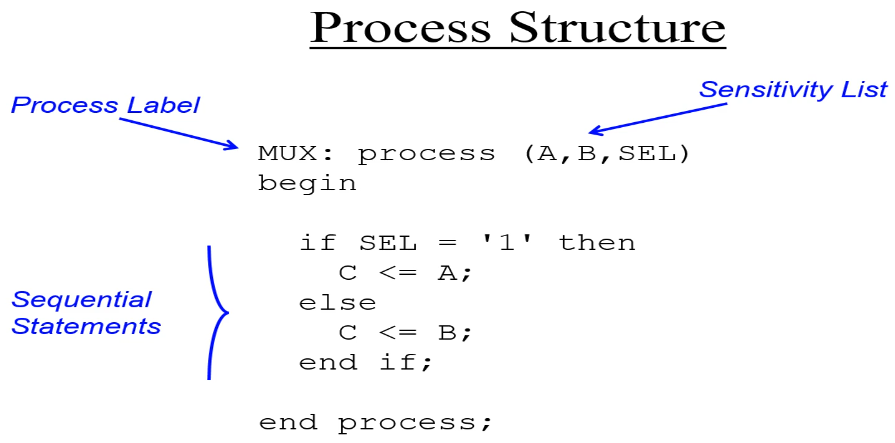
\includegraphics[scale=0.35,frame]{Figures/intro_hdl/process_syntax}
\caption{VHDL process}
\label{fig:intro_hdl:process_syntax}
\end{figure}

\begin{itemize}

\item Sensitivity list is used when a process will be executed

	\begin{itemize}
	\item It is executed when at least 1 of the input is changed
	\end{itemize}

\end{itemize}

Later we will see why we use sensitivity list in \verb|VHDL| (\autoref{sec:process_rules}). \\

\newpage
\section{Some VHDL Examples}

In this section we take some example of some \verb|VHDL| code to get more practice.

\begin{itemize}

\item \autoref{fig:intro_hdl:nor_gate} present the code of a \verb|NOR| gate

\begin{figure}[h]
\centering
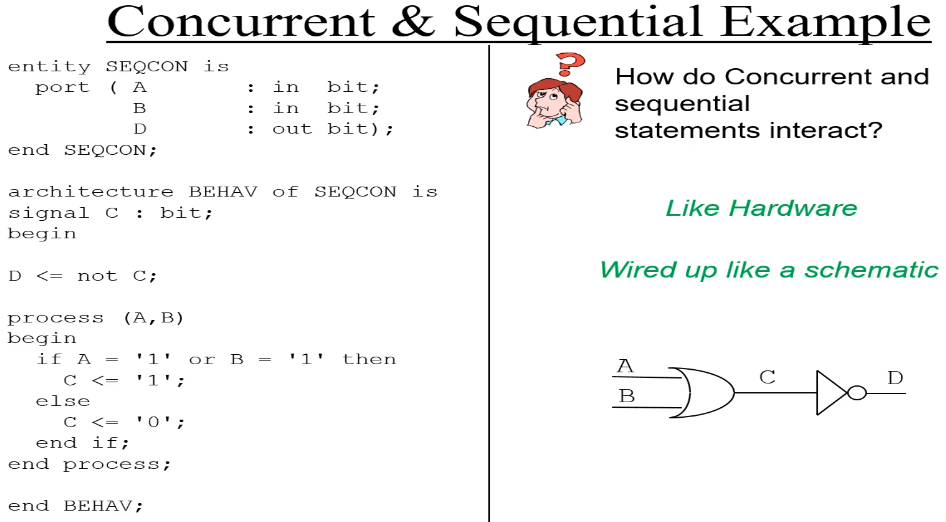
\includegraphics[scale=0.4,frame]{Figures/intro_hdl/nor_gate}
\caption{VHDL NOR gate}
\label{fig:intro_hdl:nor_gate}
\end{figure}

	\begin{itemize}
	\item Like we use wire to connect circuit in schematic, in \verb|VHDL| we use \verb|signal| to do the connection
	
	\item The code of \autoref{fig:intro_hdl:nor_gate} present an example of sequential statement interacting with concurrent statement \verb|D <= not C|
	\end{itemize}


\newpage
\item \autoref{fig:intro_hdl:vhdl_exp_2} presents an example of using 2 same statements, but one outside a process (inside the architecture), and the other inside a process 

\begin{figure}[h]
\centering
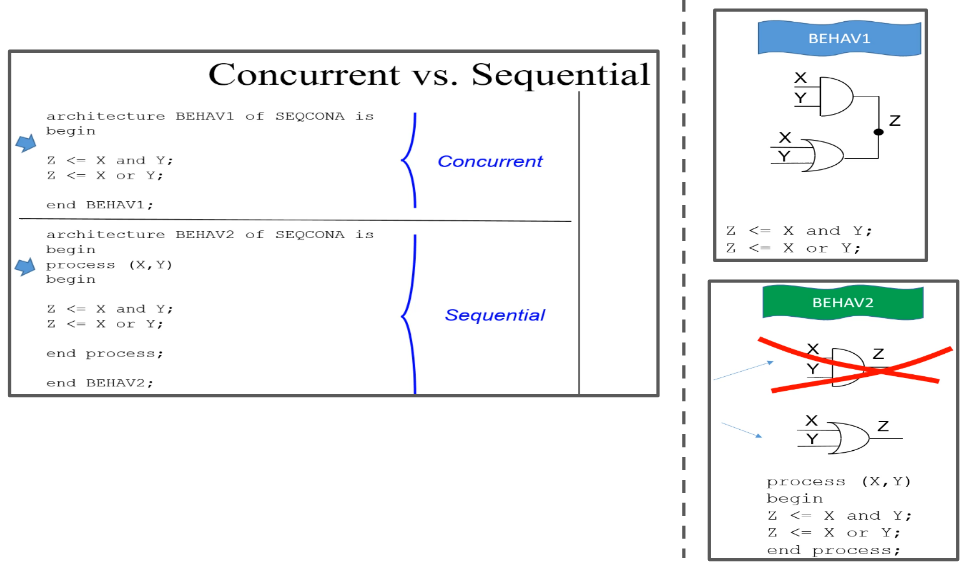
\includegraphics[scale=0.4,frame]{Figures/intro_hdl/vhdl_exp_2}
\caption{VHDL NOR gate}
\label{fig:intro_hdl:vhdl_exp_2}
\end{figure}

	\begin{itemize}
	\item This illustrate the difference between sequential and concurrent code
	
	\item In the $\mathrm{1}^\mathrm{st}$ behaviour, the same set of input (of logic) are driving the same wire. 
	
	This is isn't good because it causes a \textit{contention}
	
	\item In the $\mathrm{2}^\mathrm{nd}$ beahviour, it turns out that the first statement get ignored, and only second statment get executed
	
	
	\end{itemize}

Actually this one of the \verb|process| rules, which states that:

	\begin{itemize}
	\item Only last valid assignement to a signal takes place inside a \verb|process|
	
	\item That assignment happens at \textit{the end} of a \verb|process|
	\end{itemize}

\end{itemize}

\newpage
\section{Process Rules}
\label{sec:process_rules}

Let's see the \verb|process| rules in this section.

\begin{itemize}

\item Process executes when inputs in the sensitivity list change

\item Process can only contains sequential statements

\item Signal assignment occurs at the \textit{end} \verb|process| statment

	\begin{itemize}
	\item They don't happen when the statement get executed, they only happen at the end \verb|process|.
	
	
	\end{itemize}	 

\item Signal get the last executed assignment

\end{itemize}

These rules are a little bit of strang at first, but we will revisit them always and need to remember them, since these rules affect our way of designing our code and the sequential statement inside the \verb|process|.

\newpage
\section{More about VHDL Langugage}

Throughout our progress, we learn more \verb|VHDL| concept and features as needed, so we can grasp concept in a sequential manner.

 
\subsection{Bit Vectors}
\label{sub:bit_vectors}

First let's start with signal that are larger than 1 bit, which are \verb|bit_vector|.

\verb|bit_vector| are group of bits, or from a programming side array of bits.\\

An example is shown in \autoref{fig:intro_hdl:vhdl_vectors}.

\begin{figure}[h]
\centering
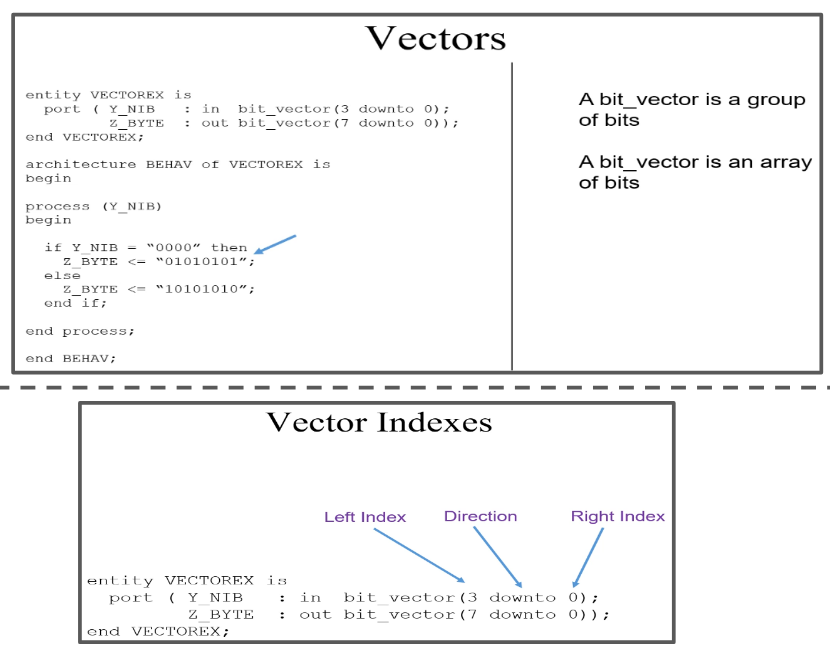
\includegraphics[scale=0.4,frame]{Figures/intro_hdl/vhdl_vectors}
\caption{Vectors variables in VHDL}
\label{fig:intro_hdl:vhdl_vectors}
\end{figure}

\begin{itemize}

\item We have \verb|Y_NIB| and \verb|Z_BYTE|, 4 and 8 bit vectors respectevely

\item Note for vectors we use double quotation \verb|""|, as opposed to signal which use single quotation \verb|''| for 1 bit case

\item For indices: they are going from left to right as shown in the $\mathrm{2}^\mathrm{nd}$ part of \autoref{fig:intro_hdl:vhdl_vectors}, with a description in the middle \verb|downto| or \verb|upto|

\end{itemize}

\newpage
\subsection{Bad code: vector mismatch}

Nice thing about \verb|VHDL| it is a strict languafe, it won't let you assign vectors to different size, or of different type. An example of bad code is shown in \autoref{fig:intro_hdl:vectors_bad_code}.

\begin{figure}[h]
\centering
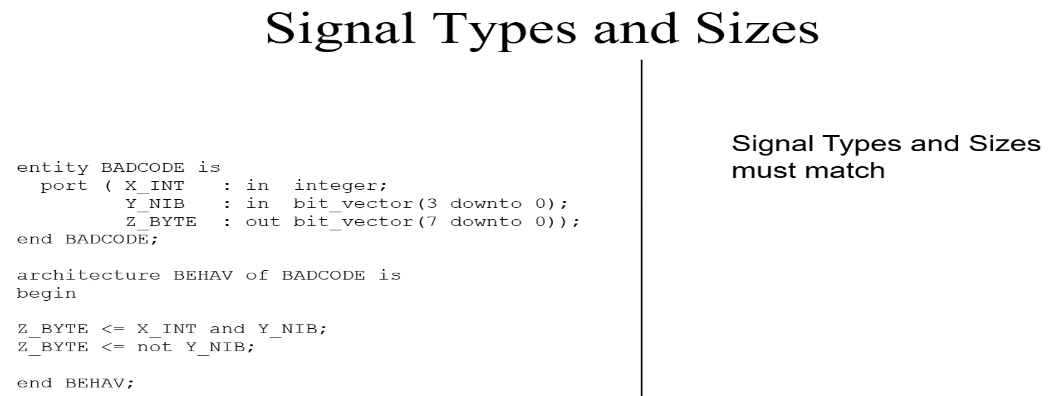
\includegraphics[scale=0.4,frame]{Figures/intro_hdl/vectors_bad_code}
\caption{Vectors bad code}
\label{fig:intro_hdl:vectors_bad_code}
\end{figure}

\begin{itemize}

\item We have 2 concurrent statements

\item The $\mathrm{1}^\mathrm{st}$ statement we get a compile time error since we are trying to assign to \verb|Z_BYTE| from 4 vector, and also a wrong type variable (\verb|X_INT| is integer)

\item The $\mathrm{2}^\mathrm{nd}$ statement is also wrong since \verb|Y_NIB| is 4 bit vector, whereas \verb|Z_BYTE| is 8 bit vector

\end{itemize}

\subsection{Code comments}

In \verb|VHDL| comments are insetered after 2 dashes \verb|--|. An example is shown in \autoref{fig:intro_hdl:vhdl_comment}.

\begin{figure}[h]
\centering
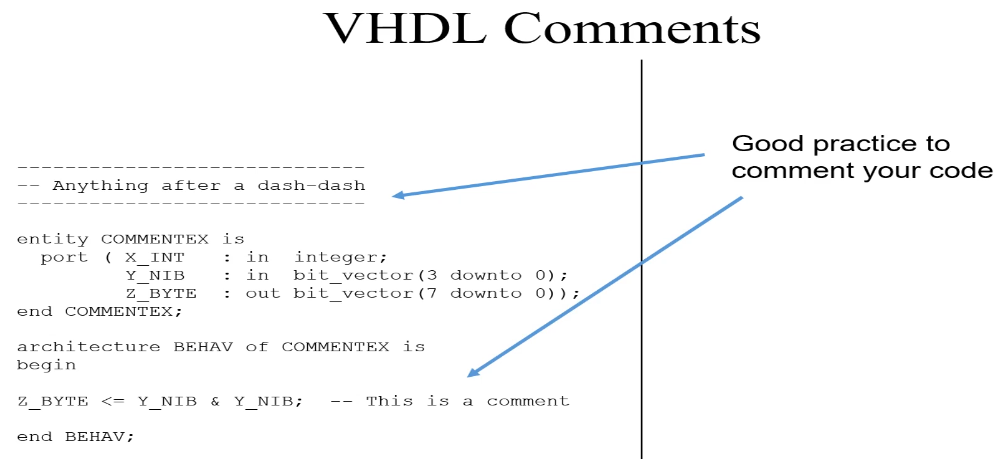
\includegraphics[scale=0.4,frame]{Figures/intro_hdl/vhdl_comment}
\caption{VHDL comment}
\label{fig:intro_hdl:vhdl_comment}
\end{figure}

However in \verb|VHDL|, there isn't a block comment feature as in some other programming language.

\subsection{VHDL syntax exercice}

\verb|VHDL| is a strict language, and we often need time and practice to get use to it. If we make some mistakes, the compiler gives errors, but it will be hard to find where these error happens, so we need to practice on the syntax and rules. \\

\underline{Given:} \autoref{fig:intro_hdl:vhdl_exercice_syntax} contains a \verb|VHDL| code with some errors. Try to spot the errors.

\begin{figure}[h]
\centering
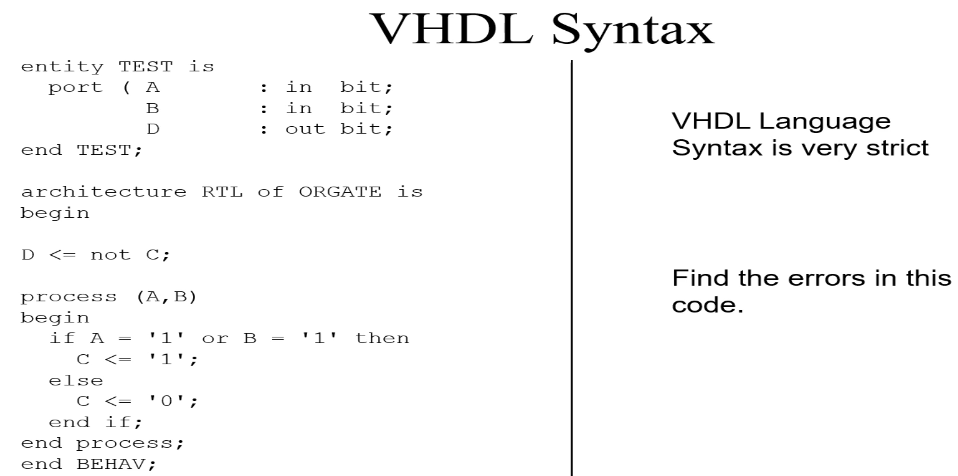
\includegraphics[scale=0.4,frame]{Figures/intro_hdl/vhdl_exercice_syntax}
\caption{VHDL syntax exercice}
\label{fig:intro_hdl:vhdl_exercice_syntax}
\end{figure}

\underline{Solution:} 

\begin{itemize}

\item $\mathrm{1}^\mathrm{st}$ error in the \verb|entity| declaration, we are missing the last parenthesis before the last semicolone 

	\begin{itemize}
	\item $\leftrightarrow$ \verb|D:out bit);|
	\end{itemize}



\item $\mathrm{2}^\mathrm{nd}$ in the \verb|architecture| we are referring to the wrong \verb|entity| name

	\begin{itemize}
	\item It should be \verb|TEST| instead of \verb|ORGATE| 
	
    \item $\leftrightarrow$ \verb|architecture RTL of TEST is|
	
	\end{itemize}

\item Signal declaration is missing for variable \verb|C|

	\begin{itemize}
	\item it should be declared after the \verb|architecture|, and before the $\mathrm{1}^\mathrm{st}$ \verb|begin| statement
	
	\item $\leftrightarrow$ \verb|signal C : bit| (see \ref{sub:internal_sig} and \autoref{fig:intro_hdl:int_sig_ex})
	\end{itemize}

\item At last, we are ending with the wrong architecture name

	\begin{itemize}
	\item it should be \verb|RTL| instead of \verb|BEAHV|
	
	\item $\leftrightarrow$ \verb|end RTL|
	\end{itemize}

\end{itemize}



\newpage
\section{Summary Introduction}

\begin{itemize}

\item Basic idea behind \verb|HDL|: give our desing some desing or behaviour, and let the tools figure out the underlying logic and gates (\ref{sec:why_hdl})

\item Desing evolution: transistor $\rightarrow$ gates and logic $\rightarrow$ \verb|HDL| (\ref{sub:desing_evolution})

\item  The output of a \verb|VHDL| (or any \verb|HDL|) is a circuit, and not a binary or some executable like known programming languages (\ref{sub:vhdl_nature})

\item Development process of an FPGA (\ref{sec:desing_flow}): we have mainly 3 steps

	\begin{enumerate}
	\item Behavioral simulation: writing code, compiling the code then verify the behaviour using a set of stimilus and visualise them  by waveforms
	
	\item Gate level simulation: which include synthesis verification, then checking if output of logic gates is correct or not
	
	\item Place and route: make the connections within and between FPGA cells (review \ref{sub:fpga_conf} for more details about connections)		
		
	\end{enumerate}


\end{itemize}

Now regarding \verb|VHDL| (\ref{sec:vhdl_desing}):

\begin{itemize}

\item From a language desing:

	\begin{itemize}
	
	\item Mainly a \verb|VHDL| program consist of 2 parts: entity and architecture
	
	\item Entity: we list input and output, and all their relative information (their types, modes,$\cdots$)
	
	\item Architecture: contains the body of our code, and consist of describing how the system work 
			
	\end{itemize}

\item For the architecture:

 \begin{itemize}
	
 \item Anything after the architecture delaration is executed in parallel 		

 \item An architecture is a combination of many processes, internal variables declaration, $\cdots$ 
 
 \item A \verb|VHDL| rule: an architecture must be associated to some entity

 \end{itemize}

\item In a \verb|process|

	\begin{itemize}
	\item all the code is executed sequentially 
	
	\item The process should contains a sensitivity list $\leftrightarrow$ \verb|process(A,B)|
	
	\item We say that this process is \textit{sensitiv} to \verb|A| and \verb|B|
	\end{itemize}


\item A \verb|VHDL| code usually consist of a combination of sequential and concurrent statement.

	\begin{itemize}
	\item Order of execution of concurrent statement is not important, since all statement are executed simulatenously, using FPGA (hardware) capacity (\ref{sub:process})
	\end{itemize}



\end{itemize}




